\documentclass[a4paper, 15pt]{article}
\usepackage[left=0.85in, right=0.85in, top=0.5in, bottom=0.95in]{geometry}
\usepackage[T1]{fontenc}
\usepackage[utf8]{inputenc}
\usepackage[italian]{babel}
\usepackage[none]{hyphenat} % no sillabazione 
\usepackage[none]{hyphenat} % no sillabazione 
\usepackage{multicol} %testo su più colonne
\usepackage{enumerate}
\usepackage{mdwlist} %suspend enumerate \suspend{} \resume{}
\usepackage{lipsum} %testo random per verifica \lipsum
\usepackage{graphicx, nicefrac}
\usepackage{wrapfig2}
\usepackage{amsmath}
\usepackage{amssymb}
\usepackage{amsthm} %teoremi e dimostrazioni e definizioni
\usepackage{cases}
\usepackage{gensymb} %simboli come ° = \degree  etc etc
\usepackage{pifont} %\cmark \xmark
\usepackage{cancel} %permette di fare semplificazioni utilizzando il comando \cancel{expression}
\usepackage{subcaption}
\usepackage{hyperref}
\hypersetup{
	colorlinks=true,
	linkcolor=blue,    
	urlcolor=blue,
	%pdfpagemode=FullScreen, %il pdf generato non si avvia a schermo intero
}
\urlstyle{same}
\usepackage{changepage}
\usepackage{lastpage, epstopdf}
\usepackage{fancyhdr}
\usepackage{tcolorbox}
\usepackage{color} % testo colorato \textcolor{'ColorCode'}{'testo'}
\usepackage[labelformat=empty]{caption} %Elimina le "figura 1" dalle caption.
\usepackage{setspace} % in questo modo posso settare lo spoazio dell'indice \begin{spacing}{0.95}
	\usepackage{tikz} %disegni e mappe
	\usetikzlibrary{patterns}
	\usepackage{pgfplots}
	\pgfplotsset{compat=1.15}
	\usepackage{mathrsfs}
	\usetikzlibrary{arrows,decorations.markings}
	\raggedbottom
	\setlength{\parindent}{0pt}
	

	
		\begin{document}
		
		
		
\section{Turbina Pelton ottimizzata}
% \begin{tikzpicture}[>=latex] [font=\itshape]	
% 	\draw [help lines] (0,0) grid (5,5);
% 	\draw [->] (1,1) -- (4,1) node [pos=0.5, sloped, below] {$u$};
% 	\draw [->] (4,1.5) -- (2.4,1.5) node [pos=0.5, sloped, above] {$w_2$};
% 	\draw [->] (1,1.5) -- (2.4,1.5) node [pos=0.5, sloped, above] {$c_2$};;
% \end{tikzpicture}

\section{RENDIMENTO PELTON} 
%\begin{tikzpicture}[line cap=round,line join=round,>=triangle 45]
%	\begin{axis}[
%		x=5cm,y=5cm,
%		axis lines=middle,
%		%		ymajorgrids=true,
%		%		xmajorgrids=true,
%		xmin=-0.05,
%		xmax=1.3,
%		ymin=0.0,
%		ymax=1.1, xticklabels=\empty,yticklabels=\empty,
%		extra x ticks={0.85, 0.85/2, 1}, extra y ticks={0.8, 1},
%		xlabel=$K_p$, ylabel=$\eta$,title={\textcolor{red}{$\beta_2=15\degree,~\varphi=0.85,~\psi=1$}  $\beta_2=15\degree,~\varphi=1,~\psi=1$}]
%		\clip(-0.05,0.) rectangle (1.05,1.05);
%		\draw [samples=50,rotate around={-180.:(0.5,0.9829629131445341)},xshift=2.5cm,yshift=4.91481456572267cm,line width=2.pt,domain=-1.271665475151249:1.271665475151249)] plot (\x,{(\x)^2/2/0.1271665475151249});
%		\draw [red, dashed, samples=50,rotate around={-180.:(0.425,0.710190704746926)},xshift=2.125cm,yshift=3.55095352373463cm,domain=-1.271665475151249:1.271665475151249)] plot (\x,{(\x)^2/2/0.1271665475151249});
%		\draw [red, dashed]  (0.85/2, 0) -- (0.85/2, {(0.85/2)^2/2/0.1271665475151249});
%		\draw [dashed]  (0.5, 0) -- (0.5,1);		
%	\end{axis}
%	\node at (2.3,-0.8) {$\varphi\over2$};
%	\node at (4.5,-0.7) {$\varphi$};
%\end{tikzpicture}
\section{Palettatura pelton}
%		\begin{tikzpicture}[>=latex] [font=\itshape]
%			\draw [help lines] (0,0) grid (5,5);
%			%Palettatura
%			\draw (5,2) arc (90:-90:0.75 and 1);	
%			\draw (5,4) arc (90:-90:0.75 and 1);
%			%Triangolo in ingresso
%			\draw [->] (2,2) -- (5,2) node [pos=0.5, sloped, above] {$c_1$};
%			\draw [->] (2,1.75) -- (3.5,1.75) node [pos=0.5, sloped, below] {$w_1$};
%			\draw [->] (3.5,1.75) -- (5,1.75) node [pos=0.5, sloped, below] {$u_1$};
%			%Triangolo in uscita
%			\draw [->] (5,0) -- (4,-0.45) node [pos=0.5, sloped, above] {$w_2$};
%			\draw [->] (4,-0.45) -- (5.5,-0.45) node [pos=0.5, sloped, below] {$u_2$};
%			\draw [->] (5,0) -- (5.5,-0.45) node [pos=0.5, sloped, above] {$c_2$};			
%		\end{tikzpicture}
\section{Generico triangolo Francis}
%	\begin{tikzpicture}[>=latex] [font=\itshape]
%		\draw [help lines] (0,0) grid (5,5);
%		\draw [->] (2,1) -- (5,1) node  [pos=0.5, sloped, below] {$u_1$};
%		\draw [->] (0,1.3) -- (5,1) node  [pos=0.5, sloped, above] {$c_1$};
%		\draw [->] (0,1.3) -- (2,1) node  [pos=0.5, sloped, below] {$w_1$};
%%		\draw [->] (1.5,1) arc (180:150:1) node  [pos=0.5, sloped, above] {$\beta_1$};
%%		\draw [dashed] (2,1) -- (1.5,1);
%%		\draw [->] (4,1) arc (180:150:1) node  [pos=0.5, sloped, above] {$\alpha_1$};
%%		\draw [->] (0, 0.5) -- (5, 0.5) node  [pos=0.5, sloped, below] {$c_{1u}$};		
%	\end{tikzpicture}

\section{Tubo Diffusore 1}
%\begin{center}
%	\begin{tikzpicture}[>=latex] [font=\itshape]
%		\draw [help lines] (0,0) grid (7,7);
%		%Monte
%		\fill[cyan!30!white] (0,5) rectangle (2,6);
%		\node at (1,5.5) {Monte};
%		%Turbina
%		\node [draw, circle] at (3,3) {T};
%		%Volume di Controllo
%		\draw [dashed] (2.55,2.55) rectangle (3.45,3.45);
%		\node at (3,3.75) {$V_C$};
%		\node at (2.55,2.2) {1};
%		\node at (3.45,2.2) {2};
%		\draw[->] (3, 2.55) -- (3, 1.55) node  [pos=1, below] {$L_u$};
%		%Valle
%		\fill[cyan!30!white] (5,1) rectangle (7,2);
%		\node at (6,1.5) {Valle};
%		%Collegamenti
%		\draw (1,5) -- (2.65,3) node  [pos=0.5, above] {a};
%		\draw (3.35,3) -- (6,2) node  [pos=0.5, above] {b};
%		%Asse
%		\draw [->] (-1,1) -- (-1,6) node [pos=1, above] {$z$};
%		%Marker
%%		\draw (-1.1,3.65) -- (-0.9,3.65);
%%		\node [align=left] at (-1.4,3.65) {$z_2$};
%%		\draw (-1.1,2) -- (-0.9,2);
%%		\node [align=left] at (-1.4,2) {$z_3$};
%		%\fill [cyan] (0,4) -- (2,4) -- (2,5) -- (0,5) -- cycle;
%	\end{tikzpicture}
%\end{center}	
\section{TUBO Diffusore 2}
% \begin{tikzpicture}[>=latex] [font=\itshape]
%	\draw [help lines] (0,0) grid (7,7);
%	\draw (0,5) -- (5,7);
%	\draw (0,3) -- (5,1);
%	\node at (-0.2,4) {2}; 
%	\node at (5.2,4) {3};
%	\draw [dashed] (0,3) -- (0,5);
%	\draw [dashed] (5,1) -- (5,7);
% \end{tikzpicture}



\section{Triangoli di velocità e portata}
% \begin{tikzpicture}[>=latex] [font=\itshape]
%	\draw [help lines] (0,0) grid (15,5);
%	%Triangolo d'ingresso
%	\draw [->] (0,0) -- (4,0) node  [pos=0.5, sloped, below] {$u_1$};
%	\draw [->] (0,4) -- (0,0) node  [pos=0.25, left] {$w_1$};
%	\node [align=left] at (-0.3,1) {$w^*_1$};
%	\draw [->] (0,4) -- (4,0) node  [pos=0.5, sloped, below] {$c_1$};
%	\draw [->] (0,2) -- (4,0) node  [pos=0.5, sloped, below] {$c^*_1$};
%	\node [draw, align=left] at (2,-1) {Diminuire la portata significa\\abbassare l'altezza del triangolo};
%	%Triangolo d'uscita 
%	\draw [->] (8,0) -- (10,1) node  [pos=0.5, sloped, below] {$u_2$};
%	\draw [->] (8,3) -- (8,0) node  [pos=0.75, left] {$w_2$};
%	\node [align=left] at (7.7,2) {$w^*_2$};
%	\draw [->] (8,3) -- (10,1) node  [pos=0.5, sloped, below] {$c_2$};
%	\draw [->] (8,3) -- (11,1.5) node  [pos=0.5, sloped, above] {$c^*_2$};
%	\draw [->] (8,1.5) -- (11,1.5) node  [pos=0.5, sloped, below] {$u^*_2$};
%	
%	\node [draw, align=left] at (9,-1) {Diminuire la portata significa\\che in uscita $c_2^*$ non è più \\ perpendicolare ad $u_2$};	
% \end{tikzpicture}

\section{Impianto pelton}
%\begin{center}
%	\begin{tikzpicture}[>=latex] [font=\itshape]
%	\draw [help lines] (0,0) grid (5,5);
%	%Monte
%	\fill[cyan!30!white] (0,4) rectangle (2,5);
%	\node at (1,4.5) {Monte};
%	%Turbina
%	\node [draw, circle] at (1,1) {T};
%	%Valle
%	\fill[cyan!30!white] (3,1) rectangle (5,2);
%	\node at (4,1.5) {Valle};
%	%Collegamenti
%	\draw (1,4) -- (1,1.35);
%	\draw (1.35,1) -- (3,1);
%	%Asse
%	\draw [->] (-1,1) -- (-1,6) node [pos=1, above] {$z$};
%	%Marker
%	\draw (-1.1,1.35) -- (-0.9,1.35);
%	\node [align=left] at (-1.4,1.35) {$z_1$};
%	\draw (-1.1,5) -- (-0.9,5);
%	\node [align=left] at (-1.4,5) {$z_m$};
%	%\fill [cyan] (0,4) -- (2,4) -- (2,5) -- (0,5) -- cycle;
%\end{tikzpicture}
% \end{center}

\section{Triangoli Kaplan}
%\begin{center}
%	\begin{tikzpicture}[>=latex] [font=\itshape]
%		\draw [help lines] (0,0) grid (15,5);
%		\draw [->] (0,5) -- (5,5) node [pos=0.5, sloped, above] {$u_{1A}$};
%		\draw [->] (0,5) -- (2,0) node [pos=0.5, sloped, below] {$c_{1A}$};
%		\draw [->] (5,5) -- (2,0) node [pos=0.5, sloped, below] {$w_{1A}$};
%		
%		
%		\draw [help lines] (0,0) grid (15,5);
%		\draw [->] (10,5) -- (13,5) node [pos=0.5, sloped, above] {$u_{1B}$};
%		\draw [->] (10,5) -- (15,0) node [pos=0.5, sloped, below] {$c_{1B}$};
%		\draw [->] (13,5) -- (15,0) node [pos=0.5, sloped, below] {$w_{1B}$};
%	\end{tikzpicture}
%\end{center}


\section{generico triangolo di velocità}
%\begin{center}
%	\begin{tikzpicture}[>=latex] [font=\itshape]
%	\draw [help lines] (0,0) grid (5,5);	
%	\draw [->] (0,0) -- (5,0) node [pos=0.5, sloped, above] {$u$};
%	\draw [->] (0,0) -- (3,4) node [pos=0.5, sloped, above] {$w$};
%	\draw [->] (3,4) -- (5,0) node [pos=0.5, sloped, above] {$c$};	
%	\draw [->] (0,-0.5) -- (3,-0.5) node [pos=0.5, sloped, above] {$w_u$};
%	\draw [->] (3,-0.5) -- (5,-0.5) node [pos=0.5, sloped, above] {$c_u$};
%	\draw [dashed] (3,-1) -- (3,5);
%	\draw [->] (0.5,0) arc (0:30:1);
%	\node at (0.6,0.5) {$\beta$};
%	\draw [->] (4.5,0) arc (180:145:1);
%	\node at (4.4,0.5) {$\alpha$};
%	\draw [dashed] [->] (5.5,0) arc (0:91:1);
%	\node at (5.7,0.5) {$\alpha^*$};
%	\draw [dashed](5,0) -- (5.75,0); 
%	\end{tikzpicture}	
%\end{center}

%\begin{center}
%	\begin{tikzpicture}[>=latex] [font=\itshape]
%		\draw [help lines] (0,0) grid (10,10);	
%		\draw [->] (0,0) -- (5,0) node [pos=0.5, sloped, above] {$u$};
%		\draw [->] (0,0) -- (7,4) node [pos=0.5, sloped, above] {$w$};
%		\draw [->] (7,4) -- (5,0) node [pos=0.5, sloped, above] {$c$};	
%		\draw [->] (0,-0.5) -- (7,-0.5) node [pos=0.5, sloped, below] {$w_u$};
%		\draw [->] (5,-1) -- (7,-1) node [pos=0.5, sloped, below] {$c_u$};
%		\draw [dashed] (5,-1) -- (5,5);
%		\draw [->] (4.5,0) arc (180:90:1);
%		\node at (4.4,0.5) {$\alpha$};
%		\draw [dashed] [->] (5.5,0) arc (0:35:1);
%		\node at (5.7,0.5) {$\alpha^*$};
%		\draw [dashed](5,0) -- (5.75,0); 
%	\end{tikzpicture}	
%\end{center}
\section{Triangolo in uscita}
% \begin{center}
% \begin{tikzpicture}[>=latex] [font=\itshape]
%		\draw [help lines] (0,0) grid (5,5);
%		\draw [->] (2.5,2) -- (0,0) node [pos=0.5, sloped, above] {$w_2$};
%		\draw [->] (2.5,2) -- (4,0) node [pos=0.5, sloped, above] {$u_2$};
%		\draw [->] (0,0) -- (4,0) node [pos=0.5, sloped, below] {$c_2$};
%		\draw [->] (0.5,0) arc (0:19:1);
%		\node at (1.3,0.3) {$\beta_2<0$};
% \end{tikzpicture}	
% \end{center}

\section{Forma della generica palettatura }
% \begin{center}
% 	\begin{tikzpicture}
% 		\draw [help lines] (0,0) grid (10,10);
% 		%Palettatura
% 		\draw [thick] (7,7) to [out=225, in=35] (3,3);
% 		%Triangolo in ingresso
% 		\draw [->] (6,8) -- (8,8) node [pos=0.5, sloped, above] {$u$};
% 		\draw [->] (8,8) -- (7,7) node [pos=0.5, sloped, below] {$w_1$};
% 		\draw [->] (6,8) -- (7,7) node [pos=0.5, sloped, below] {$c_1$};
% 		%Triangolo in uscita 
% 		\draw [->] (1,3) -- (3,3) node [pos=0.5, sloped, above] {$u$};
% 		\draw [->] (3,3) -- (1,2) node [pos=0.5, sloped, below] {$w_2$};
% 		\draw [->] (1,3) -- (1,2) node [pos=0.5, left] {$c_2$};
% 	\end{tikzpicture}
% \end{center}
 
\section{palettatura per R=0}
%  \begin{center}
% 	\begin{tikzpicture}
% 		\draw [help lines] (0,0) grid (10,10);
% 		%Palettatura
% 		\draw [thick] (5,7) to [out=0, in=0] (5,1);
% 		%Triangolo in ingresso
% 		\draw [->] (3,7) -- (5,7) node [pos=0.5, sloped, below] {$w_1$};
%
% 		%Triangolo in uscita 
% 		\draw [->] (5,1) -- (3,1) node [pos=0.5, sloped, below] {$w_2$};
% 	\end{tikzpicture}
% \end{center}

\section{ANALISI TERMODINAMICA}
%\begin{center}
%	\begin{tikzpicture}[>=latex,
%		dot/.style = {draw,fill,circle,inner sep=1pt},arrow inside/.style = {postaction=decorate,decoration={markings,mark=at position .55 with \arrow{>}}}
%		]
%		%\draw [help lines] (0,0) grid (15,15);		
%			%\draw[<->] (0,6) node[above right] {$P$} |- (6,0) node[right] {$V$};
%			%\draw[->] (0,0) node[above] {$P$} %|- (6,0) node[right] {$V$};
%			\draw[->] (0,0) -- (15,0) node [pos=1, right] {$s$};
%			\draw[->] (0,0) -- (0,15) node [pos=1, above] {$h$};
%			%ISOBARE
%			\draw (4,2) to [out=25, in=225] (9,6);
%			\node [align=right] at (9.25,6) {$P_2$};
%			\draw (4,6) to [out=25, in=225] (9,10);
%			\node [align=right] at (9.25,10) {$P_1$};
%			\draw (4,9) to [out=25, in=225] (9,13);
%			\node [align=right] at (9.25,13) {$P_0$};
%			\draw (4,11) to [out=25, in=225] (9,15);
%			\node [align=right] at (9.85,15) {$P_{00} = P_{01}$};
%			%QUALCHE NODO
%			\node[dot] (@00) at (6,12.17) {};
%			\node[dot,blue,label={right:$0$}] (@0) at (6,10.17) {};			
%			\node[dot,blue,label={right:$1$}] (@1) at (6,7.17) {};
%			\node[dot,blue,label={right:$2$}] (@2) at (6,3.17) {};			
%			%Valori sulle y
%			\draw[dashed] (@00) to (0,12.17) node [left] {$h_{01}^{\text{Re}} = h_{01} = h_{00}$};
%			\draw[dashed] (@0) to (0,10.17) node [left] {$h_0$};
%			\draw[blue, dashed] (@1) to (0,7.17) node [left] {$h_1$};
%			\draw[blue, dashed] (@2) to (0,3.17) node [left] {$h_2$};
%			\draw[blue, dashed] (1,5.17) to (0,5.17) node [left] {$h_{02}$};
%			%Valori sulle x
%			\draw[blue,dashed] (@2) to (6,0) node [below] {$s_1$};
%			%Trasformazioni Ideali
%			\draw[arrow inside] (@00) to (@0);
%			\draw[blue, arrow inside] (@0) to (@1);
%			\draw[blue, arrow inside] (@1) to (@2);
%			%Velocità
%			\draw (1,10.17) -- (1,12.17) node [pos=0.5, right] {$c_0^2\over2$};
%			\draw [blue] (1.5,7.17) -- (1.5,12.17) node [pos=0.5, right] {$c_1^2\over2$};
%			\draw [blue] (1,3.17) -- (1,5.17) node [pos=0.5, right] {$c_2^2\over2$};
%			%Valori Reali
%			\node[dot,red,label={right:$1R$}] (@1R) at (7,8) {};
%			\node[dot,red,label={right:$2R$}] (@2R) at (8.5,5.5) {};
%			%Trasformazioni reali
%			\draw[red, arrow inside] (@0) to[looseness=.7,bend right=10] (@1R);
%			\draw[red, arrow inside] (@1R) to[looseness=.7,bend right=5] (@2R);
%			%Nuovi valori su x e y
%			\draw[red, dashed] (@2R) to (0,5.5) node [left] {$h_{2R}$};
%			\draw[red, dashed] (@1R) to (0,8) node [left] {$h_{1R}$};
%			\draw[red, dashed] (1,7.5) to (0,7.5) node [left] {$h_{02R}$};
%			\draw[red, dashed] (@2R) to (8.5,0) node [below] {$s_{1R}$};
%			%Velocità 
%			\draw [red] (1,5.5) -- (1,7.5) node [pos=0.5, right] {$c_2^2\over2$};
%			\draw [red] (2,8) -- (2,12.17) node [pos=0.25, right] {$c_{1R}^2\over2$};
%			%Lavoro
%			\draw [<->] (12, 12.17) -- (12, 7.5) node [pos=0.5, right] {$l_R$};
%			\draw [loosely dotted] (1,7.5) to (12,7.5);
%			\draw [loosely dotted] (@00) to (15,12.17);
%			\draw [<->] (13, 12.17) -- (13,5.17) node [pos=0.5, right] {$l_I$};
%			\draw [loosely dotted] (1,5.17) to (13,5.17);
%			\draw [<->] (14, 12.17) -- (14,3.17) node [pos=0.5, right] {$l_{\max}$};
%			\draw [loosely dotted] (@2) to (14,3.17);
%%			\node[dot,label={right:$a$}] (@a) at (3,4) {};
%%			\node[dot,label={left:$b$}] (@b) at (1.5,4.5) {};
%%			\node[dot,label={below left:$c$}] (@c) at (2,1.5) {};
%%			\node[dot,label={right:$d$}] (@d) at (5.5,1) {};
%%			\draw[arrow inside] (@a) to[looseness=.7,bend left=20] (@b);
%%			\draw[arrow inside] (@b) to[looseness=.7,bend right=20] (@c);
%%			\draw[arrow inside] (@c) to[looseness=.7,bend right=20] (@d);
%%			\draw[arrow inside] (@d) to[looseness=.7,bend left=20] (@a);
%%			\draw[dashed] (@a) to [left] (0,4);
%%			\draw[dashed] (@c) to [left] (0,1.5);
%%			\draw (-.98,4.0) node {$P_1$};
%%			\draw (-.98,1.5) node {$P_2$};
%		
%	\end{tikzpicture}
%\end{center}


\section{Stadio Rateau}
%\begin{center}
%	\begin{tikzpicture}[>=latex,
%			dot/.style = {draw,fill,circle,inner sep=1pt},arrow inside/.style = {postaction=decorate,decoration={markings,mark=at position .55 with \arrow{>}}}
%			]
%			%\draw [help lines] (0,0) grid (15,15);		
%				%\draw[<->] (0,6) node[above right] {$P$} |- (6,0) node[right] {$V$};
%				%\draw[->] (0,0) node[above] {$P$} %|- (6,0) node[right] {$V$};
%				\draw[->] (0,0) -- (15,0) node [pos=1, right] {$s$};
%				\draw[->] (0,0) -- (0,15) node [pos=1, above] {$h$};
%				%ISOBARE
%%				\draw (4,2) to [out=25, in=225] (9,6);
%%				\node [align=right] at (9.25,6) {$P_2$};
%				\draw (4,6) to [out=25, in=225] (9,10);
%				\node [align=right] at (9.25,10) {$P_1$};
%				\draw (4,9) to [out=25, in=225] (9,13);
%				\node [align=right] at (9.25,13) {$P_0$};
%				\draw (4,11) to [out=25, in=225] (9,15);
%				\node [align=right] at (9.85,15) {$P_{00} = P_{01}$};
%				%QUALCHE NODO
%				\node[dot] (@00) at (6,12.17) {};
%				\node[dot,label={right:$0$}] (@0) at (6,10.17) {};			
%				\node[dot,label={below right:$1\equiv2$}] (@1) at (6,7.17) {};
%%				\node[dot,blue,label={right:$2$}] (@2) at (6,3.17) {};			
%				%Valori sulle y
%				\draw[dashed] (@00) to (0,12.17) node [left] {$h_{01}^{\text{Re}} = h_{01} = h_{00}$};
%				\draw[dashed] (@0) to (0,10.17) node [left] {$h_0$};
%				\draw[dashed] (@1) to (0,7.17) node [left] {$h_1=h_2$};
%%				\draw[blue, dashed] (@2) to (0,3.17) node [left] {$h_2$};
%				\draw[dashed] (1,9.17) to (0,9.17) node [left] {$h_{02}$};
%				%Valori sulle x
%				\draw[dashed] (@1) to (6,0) node [below] {$s_0=s_1$};
%				%Trasformazioni Ideali
%				\draw[arrow inside] (@00) to (@0);
%				\draw[ arrow inside] (@0) to (@1);
%				%\draw[blue, arrow inside] (@1) to (@2);
%				%Velocità
%				\draw (1,10.17) -- (1,12.17) node [pos=0.5, right] {$c_0^2\over2$};
%				\draw (1.5,7.17) -- (1.5,12.17) node [pos=0.5, right] {$c_1^2\over2$};
%				\draw (1,7.17) -- (1,9.17) node [pos=0.5, left] {$c_2^2\over2$};
%%				%Valori Reali
%%				\node[dot,red,label={right:$1R$}] (@1R) at (7,8) {};
%%				\node[dot,red,label={right:$2R$}] (@2R) at (8.5,5.5) {};
%%				%Trasformazioni reali
%%				\draw[red, arrow inside] (@0) to[looseness=.7,bend right=10] (@1R);
%%				\draw[red, arrow inside] (@1R) to[looseness=.7,bend right=5] (@2R);
%%				%Nuovi valori su x e y
%%				\draw[red, dashed] (@2R) to (0,5.5) node [left] {$h_{2R}$};
%%				\draw[red, dashed] (@1R) to (0,8) node [left] {$h_{1R}$};
%%				\draw[red, dashed] (1,7.5) to (0,7.5) node [left] {$h_{02R}$};
%%				\draw[red, dashed] (@2R) to (8.5,0) node [below] {$s_{1R}$};
%				%Velocità 
%%				\draw [red] (1,5.5) -- (1,7.5) node [pos=0.5, right] {$c_2^2\over2$};
%%				\draw [red] (2,8) -- (2,12.17) node [pos=0.25, right] {$c_{1R}^2\over2$};
%				%Lavoro
%%				\draw [<->] (12, 12.17) -- (12, 7.5) node [pos=0.5, right] {$l_R$};
%%				\draw [loosely dotted] (1,7.5) to (12,7.5);
%				\draw [loosely dotted] (@00) to (14,12.17);
%				\draw [<->] (13, 12.17) -- (13,9.17) node [pos=0.5, right] {$l_I$};
%				\draw [loosely dotted] (1,9.17) to (13,9.17);
%				\draw [<->] (14, 12.17) -- (14,7.17) node [pos=0.5, right] {$l_{\max}$};
%				\draw [loosely dotted] (@1) to (14,7.17);
%	
%		\end{tikzpicture}
%\end{center}
\section{triangoli di velocità rateau}
%\begin{center}
%		\begin{tikzpicture}[>=latex] [font=\itshape]
%%			\draw [help lines] (0,0) grid (15,5);	
%			\draw [->] (5,0) -- (0,0) node [pos=0.5, sloped, above] {$u$};
%			\draw [->] (8,3) -- (5,0) node [pos=0.5, sloped, above] {$w_1$};
%			\draw [->] (8,3) -- (0,0) node [pos=0.5, sloped, above] {$c_1$};
%			\draw [->] (11,0) -- (6,0) node [pos=0.5, sloped, above] {$u$};	
%			\draw [->] (8,3) -- (11,0) node [pos=0.5, sloped, above] {$w_2$};
%			\draw [->] (8,3) -- (6,0) node [pos=0.5, sloped, below] {$c_2$};			
%			\draw [->] (8,-0.5) -- (0,-0.5) node [pos=0.5, sloped, above] {$c_{1u}$};
%			\draw [->] (12,3) -- (12,0) node [pos=0.5, right] {$c_m=w_m$};
%			\draw [->] (8,-1) -- (5,-1) node [pos=0.5, sloped, below] {$w_{1u}$};
%			\draw [->] (8,-1) -- (11,-1) node [pos=0.5, sloped, below] {$w_{2u}$};
%			\draw [->] (6,-1.5) -- (8,-1.5) node [pos=0.5, sloped, below] {$c_{2u}$};
%			\draw [dashed] (8,3) -- (8,-1.5);
%			\draw [dashed] (8,3) -- (12,3);
%			\draw [dashed] (6,0) -- (6,-1.5);
%			\draw [dashed] (5,0) -- (5,-1);
%			\draw (5,0) -- (5.5,0);
%			\draw (5.5,0) arc (0:25:1);
%			\node at (5,0.4) {$\beta_1$};
%			\draw (10.5,0) arc (180:155:1);
%			\node at (10.1,0.4) {$\beta_2$};						
%	\end{tikzpicture}
%\end{center}

\section{ triangoli di velocità rateau ottimizzato}
%\begin{center}
%		\begin{tikzpicture}[>=latex] [font=\itshape]
%%				\draw [help lines] (0,0) grid (15,5);	
%				\draw [->] (5,0) -- (0,0) node [pos=0.5, sloped, above] {$u$};
%				\draw [->] (10,3) -- (5,0) node [pos=0.5, sloped, above] {$w_1$};
%				\draw [->] (10,3) -- (0,0) node [pos=0.5, sloped, above] {$c_1$};
%				\draw [->] (15,0) -- (10,0) node [pos=0.5, sloped, above] {$u$};	
%				\draw [->] (10,3) -- (15,0) node [pos=0.5, sloped, above] {$w_2$};
%				\draw [->] (10,3) -- (10,0) node [pos=0.5, sloped, above] {$c_2$};			
%				\draw [->] (10,-0.5) -- (0,-0.5) node [pos=0.5, sloped, above] {$c_{1u} = 2u$};
%				\draw [->] (16,3) -- (16,0) node [pos=0.5, right] {$c_m=w_m$};
%				\draw [->] (10,-1) -- (5,-1) node [pos=0.5, sloped, below] {$w_{1u}$};
%				\draw [->] (10,-1) -- (15,-1) node [pos=0.5, sloped, below] {$w_{2u}$};
%				\draw [dashed] (10,3) -- (10,-1);
%				\draw [dashed] (10,3) -- (16,3);						
%		\end{tikzpicture}
%\end{center}

\section{grafico kp reazione}
%% SE VOGLIO GLI ASSI VUOTI yticklabels=\empty,		
%	\begin{tikzpicture}[line cap=round,line join=round,>=triangle 45]
%		\begin{axis}[
%			x=5.0cm,y=5.0cm,
%			axis lines=middle,
%%			ymajorgrids=true,
%%			xmajorgrids=true,
%			xmin=0.0,
%			xmax=1.2,
%			ymin=0.0,
%			ymax=1.1,
%			xtick={0.0,0.2,...,1.0000000000000002},
%			ytick={0.0,0.2,...,1.0000000000000002},xlabel=$K_p$, ylabel=$\eta_{TS}$,title={$\alpha_1=17.5\degree$}]
%			\clip(0.,0.) rectangle (1.,1.);
%			\draw[line width=1.pt,smooth,samples=100,domain=0.0:1.0] plot(\x,{4*(\x)*(cos((17.5)/pi)-(\x))});	
%			\draw [dashed,domain=0.0:1.0] plot(\x,{(cos((17.5)/pi)^2)});			
%			\draw [dashed] ({(cos((17.5)/pi)/2)}, 0) -- ({(cos((17.5)/pi)/2)}, {(cos((17.5)/pi)^2)});
%		\end{axis}
%		%Metto i nomi delle funzioni fuori dall'ambiente axis, ora conto le coordinate nel sistema assoluto, aiutandomi con la grid che poi nasconderò
%		\node at (4.5,5.2) {$\cos^2\alpha_1$};
%		\node at (3,1) {$\cos\alpha_1\over2$};
%	\end{tikzpicture}

\section{dimensionamento rateau piano meridiano}
\newpage
%\begin{center}
%	\begin{tikzpicture}[>=latex]
%		\draw [help lines] (0,0) grid (15,15);
%		\draw [loosely dash dot] (0,0) -- (10,0);
%		\draw (0,0) -- (0,3);
%		%\draw (0,3) arc (90:270:0.5 and 3);
%		\draw (0,3) -- (9,3);
%		\draw (9,0) -- (9,3);
%		%\draw (9,3) arc (90:270:0.5 and 3);
%		\draw (0,6) -- (9,6);
%		%Statore
%		\draw [pattern=north east lines] (1,6) rectangle (2,5.75);
%		\draw (1,5) rectangle (2,5.75);
%		\node at (1.5,5.375) {S};
%		\draw [pattern=north east lines] (1,5) rectangle (2,3.25);
%		%Rotore		
%		\draw (3,5) rectangle (4,5.75);
%		\node at (3.5,5.375) {R};
%		\draw [pattern=north east lines] (3,5) rectangle (4,3);
%		%Punti
%		\node [draw, circle] at (0.5,4.5) {$0$};
%		\node [draw, circle] at (2.5,4.5) {$1$};
%		\node [draw, circle] at (4.5,4.5) {$2$};
%		%Quote
%		\draw [->] (10,0) -- (10,5) node [pos=0.5, right] {$d$};
%		\draw [<->] (10,5) -- (10,5.75) node [pos=0.5, right] {$b$};
%		\draw [->] (10.5,0) -- (10.5,5.75) node [pos=0.5, right] {$D$};
%		\draw [loosely dotted] (2,5) -- (10,5);
%		\draw [loosely dotted] (2,5.75) -- (10.5,5.75);
%	\end{tikzpicture}
%\end{center}
\section{PARZIALIZZAZIONE }
%	\begin{tikzpicture}[>=latex]
%		\draw [help lines] (0,0) grid (20,20);
%		%Albero
%		\draw (5,10) circle (1cm);
%		\draw [loosely dotted] (5,11) -- (11,11);
%		\draw [loosely dotted] (-1,15) -- (14,15);
%		\draw [loosely dotted] (-1,14) -- (14,14);
%		\draw [loosely dash dot] (5,10) -- (18,10);
%		\draw (11,11) -- (18,11);
%		\draw (11,15.25) -- (18,15.25);
%		\draw (11,10) -- (11,15.25);
%		\draw (18,10) -- (18,15.25);
%		%Cassa
%		\draw (5,10) circle (4cm);
%		\draw (5,10) circle (5cm);
%		%Palettature
%		\foreach \angle in
%		{0, 20,40,60,80,100,120,140,160,180,200,220,240,260,280,300,320,340}
%		{\draw [shift={(5,10)}, line width=20pt] (\angle:5cm) -- (\angle:4cm);}
%		%Diaframmi e palettature 
%		\draw [pattern=north east lines] (12,15.25) rectangle (13,15);
%		\draw [pattern=north east lines] (12,14) rectangle (13,11.25);
%		\draw (12,14) rectangle (13,15);
%		\node at (12.5,14.5) {S};
%		\draw [pattern=north east lines] (14,14) rectangle (15,11);
%		\draw (14,14) rectangle (15,15);
%		\node at (14.5,14.5) {R};
%		%Quote
%		\draw [<->] (-0.5,14) -- (-0.5,15) node [pos=0.5, left] {$b$};
%		\draw [<->] (-0.5,6) -- (-0.5,5) node [pos=0.5, left] {$b$};
%		\draw [<->] (-1,14.5) -- (-1,5.5) node [pos=0.5, left] {$\overline{D}$};
%		%Parzializzatore
%		\draw [dotted, shift={(5,10)}] plot [domain=-3.55:3.55] (\x, {\x});
%		\draw [dotted, shift={(5,10)}] plot [domain=-3.55:3.55] (\x, {-\x});
%		\node at (5,10.5) {$\Gamma\over2$};
%		\node at (5,9.5) {$\Gamma\over2$};
%		\filldraw[shift={(5,10)}, fill=gray!30,opacity=0.95] (135:4) arc (135:225:4) -- (225:5) arc (225:135:5) -- cycle;
%		\filldraw[shift={(5,10)}, fill=gray!30,opacity=0.95] (45:4) arc (45:-45:4) -- (-45:5) arc (-45:45:5) -- cycle;
%	\end{tikzpicture}

\section{Rateau asimmetrico}
%
% \begin{tikzpicture}[>=latex] [font=\itshape]
%	\draw [help lines] (0,0) grid (15,5);	
%	\draw [->] (5,0) -- (0,0) node [pos=0.5, sloped, above] {$u$};
%	\draw [->] (10,3) -- (5,0) node [pos=0.5, sloped, above] {$w_1$};
%	\draw [->] (10,3) -- (0,0) node [pos=0.5, sloped, above] {$c_1$};
%	\draw [->] (13.35,1) -- (8.35,1) node [pos=0.5, sloped, above] {$u$};	
%	\draw [dotted] (10,3) -- (15,0);
%	\draw [->] (10,3) -- (13.35,1) node [pos=0.5, sloped, above] {$w_2$};
%	\draw [->] (10,3) -- (8.35,1) node [pos=0.5, sloped, above] {$c_2$};			
%	\draw [->] (14,3) -- (14,1) node [pos=0.5, right] {$c_{2m}=w_{2m}$};
%	\draw [->] (-1,3) -- (-1,0) node [pos=0.5, right] {$c_{1m}=w_{1m}$};	
%	\draw (5,0) -- (5.5,0) node [pos=1, right] {$\beta_1$};
%	\draw [->](5.5,0) arc (0:15:1);	
%	\draw [->](12.85,1) arc (180:165:1) node [pos=0, below] {$\beta_2$};						
% \end{tikzpicture}


\section{Triangolo voluto }
% \begin{tikzpicture}[>=latex] [font=\itshape]
%	\draw [help lines] (0,0) grid (15,5);	
%	\draw [->] (10,0) -- (5,0) node [pos=0.5, sloped, above] {$u$};
%	\draw [->] (3,3) -- (10,0) node [pos=0.5, sloped, above] {$w_2$};
%	\draw [->] (3,3) -- (5,0) node [pos=0.5, sloped, above] {$c_2$};	
%	\draw [->] (3,-0.5) -- (5,-0.5) node [pos=0.5, sloped, below] {$c_{2u}<0$};
%	\draw [->] (11,3) -- (11,0) node [pos=0.5, right] {$c_{2m}=w_{2m}$};
%	\draw [->](10.5,0) arc (0:145:1) node [pos=0.5, below] {$\beta_2$};
%	\draw (10,0) -- (10.5,0);
%	\draw [dashed] (3,3) -- (3,-0.5);
%	\draw [dashed] (5,0) -- (5,-0.5);
%	\draw [dashed] (3,3) -- (11,3);						
% \end{tikzpicture}



\section{POST PARZIALIZZAIONE triangoli di velocità rateau ottimizzato}
%\begin{center}
%		\begin{tikzpicture}[>=latex] [font=\itshape]
%		\draw [help lines] (0,0) grid (15,5);	
%		\draw [->] (5,0) -- (0,0) node [pos=0.5, sloped, above] {$u$};
%		\draw [->] (10,3) -- (5,0) node [pos=0.5, sloped, above] {$w_1$};
%		\draw [->] (10,3) -- (0,0) node [pos=0.5, sloped, above] {$c_1$};
%		\draw [->] (15.5,1) -- (10.5,1) node [pos=0.5, sloped, above] {$u$};	
%		\draw [->] (10,3) -- (15.5,1) node [pos=0.5, sloped, above] {$w_2$};
%		\draw [->] (10,3) -- (10.5,1) node [pos=0.5, sloped, above] {$c_2$};	
%		\draw [dotted](10,3) circle (5.83cm);	
%		\draw [->] (10.5,0.5) -- (10,0.5) node [pos=0.5,below] {$c_{2u} <0$};	
%		\draw [->] (10,-0.5) -- (0,-0.5) node [pos=0.5, sloped, below] {$c_{1u} = 2u$};
%		\draw [->] (16,3) -- (16,1) node [pos=0.5, right] {$c_{2m}=w_{2m}$};
%		\draw [->] (-1,3) -- (-1,0) node [pos=0.5, right] {$c_{1m}=w_{1m}$};
%		\draw [dashed] (5,0) -- (5.5,0) node [pos=1, right] {$\beta_1$};
%		\draw [->](5.5,0) arc (0:15:1);
%		\draw [->](15.75,1) arc (0:140:1) node [pos=0.5, below] {$\beta_2$};
%		%\draw [->] (10,-1) -- (5,-1) node [pos=0.5, sloped, below] {$w_{1u}$};
%		%\draw [->] (10,-1) -- (15,-1) node [pos=0.5, sloped, below] {$w_{2u}$};
%		\draw [dashed] (10,3) -- (10,0.5);
%		\draw [dashed] (10.5,1) -- (10.5,0.5);
%		\draw [dashed] (15.5,1) -- (16,1);						
%			\end{tikzpicture}
%\end{center}

\newpage
\section{Curtis - disegno}		
%\begin{center}
%		\begin{tikzpicture}[>=latex]
%			\draw [help lines] (0,0) grid (15,15);
%			\draw [loosely dash dot] (0,0) -- (10,0);
%			\draw (0,0) -- (0,3);
%			%\draw (0,3) arc (90:270:0.5 and 3);
%			\draw (0,3) -- (9,3);
%			\draw (9,0) -- (9,3);
%			%\draw (9,3) arc (90:270:0.5 and 3);
%			\draw (0,6) -- (9,6);
%			%Statore
%			\draw [pattern=north east lines] (1,6) rectangle (2,5.75);
%			\draw (1,5) rectangle (2,5.75);
%			\node at (1.5,5.375) {S};
%			\draw [pattern=north east lines] (1,5) rectangle (2,3.25);
%			%Rotore1		
%			\draw (3,5) rectangle (4,5.75);
%			\node at (3.5,5.375) {$R_1$};
%			\draw [pattern=north east lines] (3,5) --(4,5) -- (4,4) -- (5,3) -- (3,3) -- (3,5);
%			%Rotore2
%			\draw (7,5) rectangle (8,5.75);
%			\node at (7.5,5.375) {$R_2$};
%			\draw [pattern=north west lines] (8,5) --(7,5) -- (7,4) -- (6,3) -- (8,3) -- (8,5);
%			%Deviatore
%			\draw [pattern=north east lines] (5,6) rectangle (6,5.75);
%			\draw (5,5) rectangle (6,5.75);
%			\node at (5.5,5.375) {D};
%			\draw [pattern=north east lines] (5,5) rectangle (6,3.25);
%			%Punti
%			\node [draw, circle] at (0.5,4.5) {$0$};
%			\node [draw, circle] at (2.5,4.5) {$1$};
%			\node [draw, circle] at (4.5,4.5) {$2$};
%			\node [draw, circle] at (6.5,4.5) {$3$};
%			\node [draw, circle] at (8.5,4.5) {$4$};
%%			%Quote
%%			\draw [->] (10,0) -- (10,5) node [pos=0.5, right] {$d$};
%%			\draw [<->] (10,5) -- (10,5.75) node [pos=0.5, right] {$b$};
%%			\draw [->] (10.5,0) -- (10.5,5.75) node [pos=0.5, right] {$D$};
%%			\draw [loosely dotted] (2,5) -- (10,5);
%%			\draw [loosely dotted] (2,5.75) -- (10.5,5.75);
%		\end{tikzpicture}
%\end{center}
\newpage	
\section{Curtis - Diagramma}
%\begin{center}
%	\begin{tikzpicture}[>=latex,
%				dot/.style = {draw,fill,circle,inner sep=1pt},arrow inside/.style = {postaction=decorate,decoration={markings,mark=at position .55 with \arrow{>}}}
%				]
%					\draw [help lines] (0,0) grid (15,15);		
%					\draw[->] (0,0) -- (15,0) node [pos=1, right] {$s$};
%					\draw[->] (0,0) -- (0,15) node [pos=1, above] {$h$};
%					%ISOBARE
%					\draw (4,2) to [out=25, in=225] (9,6);
%					\node [align=right] at (10.5,6) {$P_1\equiv P_2\equiv P_3 \equiv P_4$};
%					\draw (4,9) to [out=25, in=225] (9,13);
%					\node [align=right] at (9.25,13) {$P_0$};
%					%QUALCHE NODO
%					\node (@00) at (1,12.17) {};
%					\node[dot,label={right:$0$}] (@0) at (6,10.17) {};			
%					\node[dot,label={below right:$1$}] (@1) at (6,3.17) {};
%					%Valori sulle y
%					\draw[dashed] (1.5,12.17) to (0,12.17) node [left] {$h_{01} = h_{00}$};
%					\draw[dashed] (@0) to (0,10.17) node [left] {$h_0$};
%					\draw[dashed] (@1) to (0,3.17) node [left] {$h_1=h_2=h_3$};
%					\draw[dashed] (3,5.17) to (0,5.17) node [left] {$h_{02}=h_{03}$};
%					\draw[dashed] (1,4.17) to (0,4.17) node [left] {$h_{04}$};
%					%Valori sulle x
%					\draw[dashed] (@1) to (6,0) node [below] {$s_0=s_1$};
%					%Trasformazioni Ideali
%					\draw[ arrow inside] (@0) to (@1);
%					%Velocità
%					\draw (1,10.17) -- (1,12.17) node [pos=0.5, left] {$c_0^2\over2$};
%					\draw (1.5,3.17) -- (1.5,12.17) node [pos=0.5, right] {${c_1^2\over2} = h_{00}-h_1 = \Delta h_\text{stadio}$};
%					\draw (3,3.17) -- (3,5.17) node [pos=0.5, right] {${c_2^2\over2} \underset{HP}{=} {c_3^2\over2}$};
%					\draw (1,3.17) -- (1,4.17) node [pos=0.5, left] {${c_4^2\over2}_{HP}$};
%					%Lavori 
%					\draw [dotted] (1,4.17) -- (12,4.17);
%					\draw [dotted] (@1) -- (12,3.17);
%					\draw [dotted] (@00) -- (12,12.17);
%					\draw [<->] (12,3.17) -- (12,4.17) node [pos=0.5, right] {$l_{R_2}=h_{03} - h_{04} = {c_3^2\over2} - {c_4^2\over2}$};
%					\draw [<->] (12,4.17) -- (12,12.17) node [pos=0.5, right] {$l_{R_1}=h_{00} - h_{02} = {c_1^2\over2} - {c_2^2\over2}$};
%			\end{tikzpicture}
%\end{center}	
	
%	\begin{tikzpicture}[>=latex] [font=\itshape]
%		\draw [help lines] (0,0) grid (6,6);
%		\draw [<-] (3,1) -- (6,1);
%		\draw [->] (3,3) -- (6,1) node  [pos=0.5, sloped, above] {$w_2$};
%		\draw [->] (3,3) -- (3,1);
%		\draw [->] (3,3) -- (0,1) node  [pos=0.5, sloped, above] {$w_3$};
%		\draw [->] (3,0.5) -- (0,0.5) node  [pos=0.5, below] {$+w_u$};
%		\draw [->] (3,0) -- (6,0) node  [pos=0.5, below] {$-w_u$};	
%	\end{tikzpicture}

\newpage
\section{Curtis - Triangoli di velocità}
%	\begin{tikzpicture}[>=latex] [font=\itshape]
%			\draw [help lines] (0,0) grid (20,10);
%			%4
%			\draw [<-] (10,3) -- (12,3) node  [pos=0.5, sloped, below] {$u$};
%			\draw [->] (10,5) -- (12,3) node  [pos=0.5, sloped, above] {$w_4$};
%			\draw [->] (10,5) -- (10,3) node  [pos=0.5, sloped, above] {$c_4$};
%			%2
%			\draw [<-] (14,3) -- (16,3) node  [pos=0.5, sloped, below] {$u$};
%			\draw [->] (10,5) -- (14,3) node  [pos=0.75, sloped, above] {$w_2$};
%			\draw [->] (10,5) -- (16,3) node  [pos=0.75, sloped, below] {$c_2$};	
%			%3
%			\draw [<-] (6,3) -- (8,3) node  [pos=0.5, sloped, below] {$u$};
%			\draw [->] (10,5) -- (8,3) node  [pos=0.5, sloped, above] {$w_3$};
%			\draw [->] (10,5) -- (6,3) node  [pos=0.65, sloped, below] {$c_3$};
%			%1
%			\draw [<-] (2,3) -- (4,3) node  [pos=0.5, sloped, below] {$u$};
%			\draw [->] (10,5) -- (4,3) node  [pos=0.85, sloped, above] {$w_1$};
%			\draw [->] (10,5) -- (2,3) node  [pos=0.75, sloped, above] {$c_1$};
%			%Distanze 
%			\draw [<->] (4,2.5) -- (6,2.5) node  [pos=0.5, sloped, below] {$u$};
%			\draw [<->] (8,2.5) -- (10,2.5) node  [pos=0.5, sloped, below] {$u$};
%			\draw [<->] (12,2.5) -- (14,2.5) node  [pos=0.5, sloped, below] {$u$};
%		\end{tikzpicture}
\newpage

\section{Irreversibilità}
%\begin{center}
%	\begin{tikzpicture}[>=latex,
%					dot/.style = {draw,fill,circle,inner sep=1pt},arrow inside/.style = {postaction=decorate,decoration={markings,mark=at position .55 with \arrow{>}}}
%					]
%						\draw [help lines] (0,0) grid (15,15);		
%						\draw[->] (0,0) -- (15,0) node [pos=1, right] {$s$};
%						\draw[->] (0,0) -- (0,15) node [pos=1, above] {$h$};
%						%ISOBARE
%						\draw (4,2) to [out=25, in=225] (9,6);
%						\node [align=right] at (10.5,6) {$P_1$};
%						\draw (4,9) to [out=25, in=225] (9,13);
%						\node [align=right] at (9.25,13) {$P_0$};
%						%QUALCHE NODO
%						\node (@00) at (1,12.17) {};
%						\node[dot,label={right:$0$}] (@0) at (6,10.17) {};			
%						\node[dot,label={below right:$1$}] (@1) at (6,3.17) {};
%						\node[dot,label={below right:$1R$}, red] (@1R) at (7,4) {};
%						%Valori sulle y
%						\draw[dashed] (2,12.17) to (0,12.17) node [left] {$h_{01} = h_{00}$};
%						\draw[dashed] (@0) to (0,10.17) node [left] {$h_0$};
%						\draw[dashed] (@1) to (0,3.17) node [left] {$h_1$};
%						\draw[dashed, red] (@1R) to (2,4);
%						%Valori sulle x
%						\draw[dashed] (@1) to (6,0) node [below] {$s_0=s_1$};
%						%Trasformazioni Ideali
%						\draw[ arrow inside] (@0) to (@1);
%						%Trasformazioni Reali
%						\draw[arrow inside, red] (@0) to[looseness=.7,bend right=10] (@1R);
%						%Velocità
%						\draw (1,10.17) -- (1,12.17) node [pos=0.5, left] {$c_0^2\over2$};
%						\draw (1.5,3.17) -- (1.5,12.17) node [pos=0.5, right] {${c_1^2\over2}$};
%						\draw [red] (2,4) -- (2,12.17) node [pos=0.5, right] {${c_{1R}^2\over2}$};
%						%Nomi
%						\draw [dotted] (@1) -- (10,3.17); 
%						\draw [dotted] (@1R) -- (10,4); 
%						\draw [<->, red] (10,3.17) -- (10,4) node [pos=0.5, right] {Perdite}; 
%				\end{tikzpicture}
%\end{center}
\newpage
\section{Azione - diagramma}
%\begin{center}
%	\begin{tikzpicture}[>=latex,
%				dot/.style = {draw,fill,circle,inner sep=1pt},arrow inside/.style = {postaction=decorate,decoration={markings,mark=at position .55 with \arrow{>}}}
%				]
%				\draw [help lines] (0,0) grid (15,15);		
%					\draw[->] (0,0) -- (15,0) node [pos=1, right] {$s$};
%					\draw[->] (0,0) -- (0,15) node [pos=1, above] {$h$};
%					%ISOBARE
%					\draw (4,2) to [out=25, in=225] (9,6);
%					\node [align=right] at (9.25,6) {$P_2$};
%					\draw (4,6) to [out=25, in=225] (9,10);
%					\node [align=right] at (9.25,10) {$P_1$};
%					\draw (4,9) to [out=25, in=225] (9,13);
%					\node [align=right] at (9.25,13) {$P_0$};					
%					%QUALCHE NODO
%					\node (@00) at (6,12.17) {};
%					\node[dot,label={right:$0$}] (@0) at (6,10.17) {};			
%					\node[dot,label={below right:$1$}] (@1) at (6,7.17) {};
%					\node[dot,label={right:$2$}] (@2) at (6,3.17) {};
%					\node[dot,red,label={right:$2R$}] (@2R) at (7.5,4.50) {};
%					\node[dot,red,label={right:$1R$}] (@1R) at (6.47,7.55) {};			
%					%Valori sulle y
%					\draw[dashed] (@00) to (0,12.17) node [left] {$h_{01} = h_{00}$};
%					\draw[dashed] (@0) to (0,10.17) node [left] {$h_0$};
%					\draw[dashed] (@1) to (0,7.17) node [left] {$h_1$};
%					\draw[dashed] (@2) to (0,3.17) node [left] {$h_2$};
%					%Valori sulle x
%					\draw[dashed] (@1) to (6,0) node [below] {$s_{0,1,2}$};
%					\draw[dashed,red] (@2R) to (7.5,0) node [below] {$s_{2R}$};
%					\draw[dashed,red] (@1R) to (6.47,-0.25) node [below] {$s_{1R}$};
%					%Trasformazioni Ideali
%					\draw[arrow inside] (@0) to (@1);
%					\draw[arrow inside] (@1) to (@2);
%					%Velocità
%					\draw (1,10.17) -- (1,12.17) node [pos=0.5, right] {$c_0^2\over2$};
%					\draw (1.5,7.17) -- (1.5,12.17) node [pos=0.5, right] {$c_1^2\over2$};
%					\draw [red] (2,4.5) -- (2,6.5) node [pos=0.75, right] {$c_2^2\over2$};
%					\draw (1,3.17) -- (1,5.17) node [pos=0.5, right] {$c_2^2\over2$};
%					%Trasformazioni reali
%					\draw[red, arrow inside] (@0) to[looseness=.7,bend right=10] (@2R);
%					%Lavoro
%					\draw [dashed] (@00) to (12,12.17);
%					\draw [red, dashed] (@2R) to (2,4.5);
%					\draw [red, dashed] (2,6.5) to (11,6.5);
%					\draw [dashed] (1,5.17) to (12,5.17);
%					\draw [<->] (12, 12.17) -- (12,5.17) node [pos=0.5, right] {$l_I = h_{00}-h_{02}\ne {c_1^2\over2}$};
%					\draw [red, <->] (11, 6.5) -- (11,12.17) node [pos=0.5, right] {$l_R$};		
%			\end{tikzpicture}
%\end{center}
\newpage
\section{Azione - grandezze}
%\begin{center}
%	\begin{tikzpicture}[>=latex]
%		\draw [help lines] (0,0) grid (15,15);
%		\draw[->] (0,0) -- (10,0) node [pos=1, right] {$x$};
%		\draw[->] (0,0) -- (0,10) node [pos=0, below] {$0$};
%		\draw (5,10) -- (5,0) node [pos=1, below] {$1$};
%		\node at (10,-0.2) {2};
%		\node at (2.5,-0.2) {Statore};
%		\node at (7.5,-0.2) {Rotore};
%		%H0
%		\draw[teal, thick] (5,8) to (0,8) node [left] {$\text{Entalpia Totale} ~ h_{0}$}; 
%		\draw[teal, thick] (5,8) to (10,6);
%		\draw[teal, thick, <->] (11,6) -- (11,8) node [pos=0.5, right] {Lavoro estratto};
%		%H
%		\draw[violet, thick] (10,4) to (0,6) node [left] {$\text{Entalpia Statica} ~ h$}; 
%		%c
%		\draw[blue, thick] (5,7) to (0,4) node [left] {$\text{Velocità} ~ c$}; 
%		\draw[blue, thick] (5,7) to (10,5);		
%		%w
%		\node [red] at (-0.95,2)  {$\text{Velocità} ~ w$}; 
%		\draw[red, thick] (5,2) -- (10,4.5) node [pos=0.5, sloped, below] {Espansione del fluido}; 
%		%NB
%		\node [rounded corners=1ex, draw]
%		at (5,-1) {NB: Il condotto rotorico è un condotto accelerante: $w_2>w_1$};
%	\end{tikzpicture}
%\end{center}
\newpage

\section{Azione - Triangoli}
%Generico
%\begin{tikzpicture}[>=latex]
%		\draw [help lines] (0,0) grid (10,10);
%		%2
%		\draw [->] (10,0) -- (7,0) node [pos=0.5, sloped, below] {$u$};
%		\draw [->] (5,4) -- (7,0) node [pos=0.75, sloped, below] {$c_2$};
%		\draw [->] (5,4) -- (10,0) node [pos=0.5, sloped, below] {$w_2$};
%		%1
%		\draw [->] (3,0) -- (0,0) node [pos=0.5, sloped, below] {$u$};
%		\draw [->] (5,4) -- (0,0) node [pos=0.5, sloped, below] {$c_1$};
%		\draw [->] (5,4) -- (3,0) node [pos=0.75, sloped, below] {$w_1$};
%		%Angoli
%		\draw [dotted] (3,0) -- (3.5,0);
%		\draw [->](3.5,0) arc (0:35:1) node [pos=0.5, right] {$\beta_1$};	
%		\draw [dotted] (6.5,0) -- (7,0);
%		\draw [->](6.5,0) arc (180:145:1) node [pos=0.5, left] {$\alpha_2$}; 
%		\draw [->](0.5,0) arc (0:20:1) node [pos=0.5, right] {$\alpha_1$}; 
%		\draw [->](0.4,0) arc (0:19:1);
%		\draw [->](9.6,0) arc (180:161:1) node [pos=0.5, left] {$\beta_2$}; 
%		\draw [->](9.5,0) arc (180:160:1);
%		%Lati 
%		\node at (2,1.61) {\textbf{/}};
%		\node at (8,1.61) {\textbf{/}};
%		\node [rotate=45] at (4,2) {\textbf{//}};
%		\node at (6,2) {\textbf{//}};
%\end{tikzpicture}

%Ottimizzato
%\begin{tikzpicture}[>=latex]
%	\draw [help lines] (0,0) grid (10,10);
%	%2
%	\draw [->] (8,0) -- (5,0) node [pos=0.5, sloped, below] {$u$};
%	\draw [->] (5,5) -- (5,0) node [pos=0.5, right] {$c_2$};
%	\draw [->] (5,5) -- (8,0) node [pos=0.5, sloped, below] {$w_2$};
%	%1
%	\draw [->] (5,0) -- (2,0) node [pos=0.5, sloped, below] {$u$};
%	\draw [->] (5,5) -- (2,0) node [pos=0.5, sloped, below] {$c_1$};
%	\draw [->] (5,5) -- (5,0) node [pos=0.5, left ] {$w_1$};
%
%\end{tikzpicture}

\newpage

\section{Svergolamento}

%Individuazuione del diametro medio
%\begin{tikzpicture}[>=latex]
%			\draw [help lines] (0,0) grid (15,15);
%			\draw [loosely dash dot] (0,0) -- (10,0);
%			\draw (0,0) -- (0,3);
%			%\draw (0,3) arc (90:270:0.5 and 3);
%			\draw (0,3) -- (9,3);
%			\draw (9,0) -- (9,3);
%			%\draw (9,3) arc (90:270:0.5 and 3);
%			\draw (0,6) -- (9,6);
%			%Statore
%			\draw [pattern=north east lines] (1,6) rectangle (2,5.75);
%			\draw (1,5) rectangle (2,5.75);
%			\node at (1.5,5.375) {S};
%			\draw [pattern=north east lines] (1,5) rectangle (2,3.25);
%			%Rotore		
%			\draw (3,5) rectangle (4,5.75);
%			\node at (3.5,5.375) {R};
%			\draw [pattern=north east lines] (3,5) rectangle (4,3);
%			%Punti
%			\node [draw, circle] at (0.5,4.5) {$0$};
%			\node [draw, circle] at (2.5,4.5) {$1$};
%			\node [draw, circle] at (4.5,4.5) {$2$};
%			%Quote
%			\draw [->] (10,0) -- (10,5) node [pos=0.5, right] {$d$};
%			\draw [<->] (10,5) -- (10,5.75) node [pos=0.5, right] {$b$};
%			\draw [->] (10.5,0) -- (10.5,5.75) node [pos=0.5, right] {$D$};
%			\draw [->] (9.5,0) -- (9.5,5.375) node [pos=0.5, right] {$\bar{D}$};
%			\draw [loosely dotted] (2,5) -- (10,5);
%			\draw [loosely dotted] (2,5.75) -- (10.5,5.75);
%			\draw [loosely dotted] (4,5.375) -- (9.5,5.375);
%		\end{tikzpicture}


%Traiettoria della particella
%\begin{tikzpicture}[>=latex]
%				\begin{axis}
%					[view={10}{20},axis equal, yticklabels=\empty, xticklabels=\empty, zticklabels=\empty, axis line style={draw=none}, tick style={draw=none}, ]
%					\addplot3 [shift={(2,2,2)}, rotate = 90]
%					[domain=0:15.5*pi,variable=\t,
%					samples=200,samples y=0,
%					smooth,thick,blue]
%					({cos(deg(t))},{sin(deg(t))},
%					{2*t/(6*pi)});
%					\draw [->] (0,-5,0) -- (0, 0, 0) node [pos=0.5, right] {$c_u$};
%					\draw [->] (0,-5,0) -- (2, -5, 0) node [pos=1, right] {$c_m$};
%					\draw [->] (0,-5,0) -- (0, -5, 2) node [pos=0.5, left] {$c_r$};										
%				\end{axis}				
%\end{tikzpicture}

%Traiettoria circolare
%\begin{tikzpicture}[>=latex]
%				\draw [help lines] (0,0) grid (10,10);
%				\draw [dashed] (5,5) circle (4cm);
%				\draw [dotted] (5,5) circle (5cm);
%				\draw [dotted] (5,5) circle (3cm);
%				\draw [->] (5,5) -- (2,5) node [pos=0.5, below] {$r$};
%				\draw [->] (5,5) -- (0,5) node [pos=1, left] {$r+dr$};
%				\draw (7,9.57) arc (0:180:2 and 0.43);
%				\draw (6,7.80) arc (0:175:1 and 0.2);
%				\draw (6,7.80) -- (7,9.57); 
%				\draw (4,7.80) -- (3,9.57); 
%				\node at (5,9.5) {$dm$};
%				\draw [->] (5,11) -- (5,10) node [pos=0, above] {$P+dP$};
%				\draw [->] (5,7) -- (5,8) node [pos=0, below] {$P$};
%				\draw [->] (2.5,7.7) -- (3.5,8.7) node [pos=0, below] {$P + {dP\over2}$};
%				\draw [->] (7.5,7.7) -- (6.5,8.7) node [pos=0, below] {$P + {dP\over2}$};
%				\draw [dashed] (6,7.80) -- (5,5);
%				\draw [dashed] (4,7.80) -- (5,5);
%				\draw (5.35,6) to [out=90, in=90] (4.65,6);
%				\node at (5,5.8) {$d\theta$};				
%\end{tikzpicture}

\newpage

\section{Architettura turbine}
% PIu corpi turbina
%		\begin{tikzpicture}[>=latex]
%				%\draw [help lines] (0,0) grid (15,15);
%				% HP
%				\draw [cyan, ->] (0,13) -- (0,11);
%				\draw (0,11) -- (0,10) -- (3,9) -- (3,12) -- cycle;
%				% MP
%				\draw (5,9) -- (5,12) -- (7,11) -- (7,10) -- cycle;
%				\draw (9,9) -- (9,12) -- (7,11) -- (7,10) -- cycle;
%				\draw [line width=3pt] (3, 10.5) -- (5, 10.5);
%				% Circuito vapore
%				\draw [cyan] (3,9) -- (3,8) -- (7,8);
%				\draw [cyan, ->] (7,8) -- (7,10);
%				\draw [cyan] (5,12) -- (5,13) -- (9,13);
%				\draw [cyan] (9,12) -- (9,13);
%				\draw [cyan, ->] (9,13) -- (11,13);
%				% NOMI
%				\node at (1.5,10.5) {HP};
%			\end{tikzpicture}


% Dischi e diaframmi
%\begin{center}
%	\begin{tikzpicture}[>=latex]
%			%\draw [help lines] (0,0) grid (10,10);
%			\draw [loosely dash dot] (0,0) -- (5,0);
%			% Albero
%			\draw (0,0) -- (0,0.5) -- (5,0.5) -- (5,0);
%			% Cassa
%			\draw [line width=1.5pt] (0,4.5) -- (5,6.5);
%			% Incastri
%			\draw [fill=black](0.3,4.5) -- (0.3,4.6) -- (1,4.9) -- (1,4.8) -- cycle;
%			
%			% Diaframmi
%			\draw [fill=red](0.4,3.35) -- (0.4,1) -- (0.8,1) -- (0.8,3.17) -- cycle;
%			
%			% Disco
%			\draw [fill=red] (2.2,0.5) rectangle (3,0.75);
%			\draw [fill=red] (2.4,2.72) -- (2.4,0.75) -- (2.8,0.75) -- (2.8,2.57) -- cycle;
%			
%			% Statore
%			\draw (0,3.52) -- (0,4.36) -- (1.3,4.92) -- (1.3,2.96)  -- cycle;
%			\node at (0.5,4) {S};
%			% Rotore
%			\draw (1.7,2.96) -- (1.7,4.92) -- (3.3,5.48) -- (3.3,2.4)  -- cycle;					
%			\node at (2.5,4) {R};
%		\end{tikzpicture}
%\end{center}

% A tamburo
%\begin{center}
%\begin{tikzpicture}[>=latex]
%	%\draw [help lines] (0,0) grid (10,10);
%	\draw [loosely dash dot] (0,0) -- (5,0);
%	% Albero
%	\draw (0,0) -- (0,0.5) -- (5,0.5) -- (5,0);
%	% Cassa
%	\draw [line width=1.5pt] (0,4.5) -- (5,6.5);
%	% Incastri
%	\draw [fill=black](0.3,4.5) -- (0.3,4.6) -- (1,4.9) -- (1,4.8) -- cycle;
%	
%	% Tamburo
%	\draw [line width=2pt, red](0.4,0.5) -- (0.4,3) -- (4.8,1.5) -- (4.8,0.5);
%	
%	% Disco
%	\draw [fill=red] (2.4,2.72) -- (2.4,2.35) -- (2.8,2.20) -- (2.8,2.57) -- cycle;
%	
%	% Statore
%	\draw (0,3.52) -- (0,4.36) -- (1.3,4.92) -- (1.3,2.96)  -- cycle;
%	\node at (0.5,4) {S};
%	% Rotore
%	\draw (1.7,2.96) -- (1.7,4.92) -- (3.3,5.48) -- (3.3,2.4)  -- cycle;					
%	\node at (2.5,4) {R};
%\end{tikzpicture}
%%\end{center}

%perdite di Vapore
%\begin{center}
%	\begin{tikzpicture}[>=latex]
%				%\draw [help lines] (0,0) grid (10,10);
%				\draw [loosely dash dot] (0,0) -- (5,0);
%				% Albero
%				\draw (0,0) -- (0,0.5) -- (5,0.5) -- (5,0);
%				% Cassa
%				\draw [line width=1.5pt] (0,4.5) -- (5,6.5);
%				% Incastri
%				\draw [fill=black](0.3,4.5) -- (0.3,4.6) -- (1,4.9) -- (1,4.8) -- cycle;
%				
%				% Diaframmi
%				\draw [fill=red](0.4,3.35) -- (0.4,1) -- (0.8,1) -- (0.8,3.17) -- cycle;
%				
%				% Disco
%				\draw [fill=red] (2.2,0.5) rectangle (3,0.75);
%				\draw [fill=red] (2.4,2.72) -- (2.4,0.75) -- (2.8,0.75) -- (2.8,2.57) -- cycle;
%				
%				%Vapore 
%				\pattern [pattern=north east lines,
%				pattern color=cyan] (1,1) -- (1,2.7) -- (2,2.7) -- (2,1) -- (1,1);
%				
%				% Statore
%				\draw (0,3.52) -- (0,4.36) -- (1.3,4.92) -- (1.3,2.96)  -- cycle;
%				\node at (0.5,4) {S};
%				% Rotore
%				\draw (1.7,2.96) -- (1.7,4.92) -- (3.3,5.48) -- (3.3,2.4)  -- cycle;					
%				\node at (2.5,4) {R};
%			\end{tikzpicture}
%\end{center}

%Schema appoggio appoggio

%\begin{tikzpicture}[>=latex]
%	%\draw [help lines] (0,0) grid (5,5);
%	\draw (0,0) -- (0.5,-0.5) -- (-0.5,-0.5) -- cycle;
%	\pattern [pattern=north east lines] (-0.5,-0.5) -- (0.5,-0.5) -- (0.5,-0.6) -- (-0.5,-0.6) -- cycle;
%	
%	\draw (5,0) -- (5.5,-0.5) -- (4.5,-0.5) -- cycle;
%	\node [draw, circle] at (4.7,-0.67) {};
%	\node [draw, circle] at (5.3,-0.67) {};
%	\draw (5.5,-0.85) -- (4.5,-0.85);
%	\pattern [pattern=north east lines] (5.5,-0.85) -- (4.5,-0.85) -- (4.5,-0.95) -- (5.5,-0.95) -- cycle;
%	
%	\draw (0,0) -- (5,0);
%	\draw (0,0) to[bend right=10] (5,0);
%	\draw (0,0) to[bend left=10] (5,0);
%	\draw [<-] (1.5,0) ++(45:7mm) arc (45:225:7mm);
%\end{tikzpicture}
 
 
 %Tenute a labirinto
 
%\begin{tikzpicture}[>=latex]
%%\draw [help lines] (0,0) grid (15,5);
%\draw [pattern=north east lines] (0,-1) -- (0,0) -- (2,0) -- (2,2) -- (3,2) -- (3,0) -- (6,0) -- (6,2) -- (7,2) -- (7,0) --(10,0) -- (10,-1) -- cycle;
%
%\draw [pattern=north east lines] (0,5) -- (0,1) -- (1,1) -- (1,4) -- (4,4) -- (4,1) -- (5,1) -- (5,4) -- (8,4) -- (8,1) -- (9,1) --(9,5) -- cycle;
%\end{tikzpicture}

%Generico triangolo
%\begin{tikzpicture}[>=latex]
%	\draw [help lines] (0,0) grid (10,10);
%	%2
%	\draw [->] (10,0) -- (7,0) node [pos=0.5, sloped, below] {$u$};
%	\draw [->] (5,4) -- (7,0) node [pos=0.75, sloped, below] {$c_2$};
%	\draw [->] (5,4) -- (10,0) node [pos=0.5, sloped, below] {$w_2$};
%	%1
%	\draw [->] (3,0) -- (0,0) node [pos=0.5, sloped, below] {$u$};
%	\draw [->] (5,4) -- (0,0) node [pos=0.5, sloped, below] {$c_1$};
%	\draw [->] (5,4) -- (3,0) node [pos=0.75, sloped, below] {$w_1$};
%\end{tikzpicture}

% Tcurva caratteristica
%\begin{tikzpicture}
%\draw [help lines] (0,0) grid (5,5);
%\draw[->] (0,0) -- (5,0) node [pos=1, right] {$\Psi$};
%\draw[->] (0,0) -- (0,5) node [pos=1, above] {$\Phi$};
%\draw (1,0) -- (5,5);
%\draw (0.5,1) .. controls (2.3,2) and
%(4.1,3) .. (4,5);
%\draw[dashed] (3.3,2.85) -- (3.3,0) node [pos=1, below] {$\Phi_{nom}$};
%\end{tikzpicture}


%\begin{center}
%	\begin{tikzpicture}[>=latex]
%			\draw [help lines] (0,0) grid (15,15);
%			\draw [loosely dash dot] (0,1.5) -- (5,1.5);
%			\draw (0,1.5) -- (0,3) -- (0,3) -- (5,3) -- (5,1.5);
%			\draw (0,6) -- (5,6);
%			%Statore
%			\draw [pattern=north east lines] (1,6) rectangle (2,5.75);
%			\draw (1,5) rectangle (2,5.75);
%			\node at (1.5,5.375) {S};
%			\draw [pattern=north east lines] (1,5) rectangle (2,3.25);
%			%Rotore		
%			\draw (3,5) rectangle (4,5.75);
%			\node at (3.5,5.375) {R};
%			\draw [pattern=north east lines] (3,5) rectangle (4,3);
%			%Punti
%			\node [draw, circle] at (0.5,4.5) {$0$};
%			\node [draw, circle] at (2.5,4.5) {$1$};
%			\node [draw, circle] at (4.5,4.5) {$2$};			
%		\end{tikzpicture}
%\end{center}

%\begin{tikzpicture}
%	\draw[->] (0,0) -- (5,0) node [pos=1, right] {$\dot{m}$};
%	\draw[->] (0,0) -- (0,5) node [pos=1, above] {$P_0$};
%	\draw[bend left]  (0,0) to (1,1);
%	\draw[dashed] (0,1) -- (1,1);
%	\draw[dashed] (1,0) -- (1,1);
%	\draw (1,1) -- (5,3) node [pos=0.5, sloped, above] {Bloccaggio};
%\end{tikzpicture}

%\begin{tikzpicture}
%	%\draw [help lines] (0,0) grid (5,5);
%	%x
%	\draw[->] (0,0) -- (5,0) node [pos=1, above] {$\dot{m}_{co}$};
%	%y
%	\draw[->] (0,0) -- (0,5) node [pos=1, right] {$\beta$};
%	\draw[thick] (4,0) -- (4,5);
%	\draw[bend right]  (3,1) to (4,2);
%	\draw[bend right]  (2,1) to (4,3);
%	\draw[bend right]  (1,1) to (4,4);
%	\draw[->] (3,1) -- (2,2) node [pos=1, above] {$n_{co}$};
%\end{tikzpicture}


%% Immagine hs
%\tikzset{immagine/.style={%
%		above right, inner sep=0pt, outer sep=0pt},
%	testo/.style={fill=white, align=center,
%		fill opacity=0.6, text opacity=1, below,
%		font=\sffamily\bfseries\footnotesize}}
%\begin{tikzpicture} [>=latex, red, thick]
%	\node [immagine] at (0,0)
%	{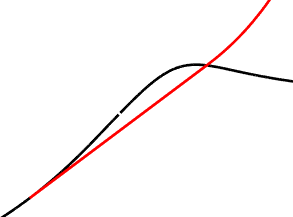
\includegraphics[width=4cm]{hs_generico(1)}};
%	\draw [help lines,step=.5] (0,0) grid (5,5);
%	%x
%	\draw[->,black] (0,0) -- (5,0) node [pos=1, above] {$s$};
%	%y
%	\draw[->,black] (0,0) -- (0,5) node [pos=1, right] {$h$};
%	\draw (3.68,3) -- (3.68,1.7) node [pos=1, right] {$h_2$};
%	\node at (4,3) {$h_1$};
%	\draw (3.68,1.7) -- (0.4,0.25) node [pos=1, left] {$h_0$};	
%\end{tikzpicture}
%
%	\scalebox{0.4}{\begin{tikzpicture}[>=latex]
%	%\draw [help lines] (0,0) grid (15,15);
%	% Generatore di Vapore con economizzatore
%	\draw (2,9) rectangle (4,11);
%	\draw [pattern=vertical lines] (2,8) rectangle (4,9);
%	% Surriscaldatore e collegamento turbina
%	\draw (3,11) -- (3,11.5) -- (3.5,12) -- (2.5,12.5) -- (3,13) -- (3,14) -- (9,14) -- (9,11);
%	% Turbina
%	\draw (9,11) -- (10,12) -- (10,9) -- (9,10) -- (9,11) -- cycle;
%	\draw [line width=3pt] (10, 10.5) -- (11, 10.5);
%	\node [draw, circle] at (11.35, 10.5) {$\sim$};
%	\draw (10,9) -- (10,8);
%	% Condensatore
%	\draw (10,7.5) circle (0.5cm);
%	\draw (11,8) -- (10,7.5) -- (11,7);
%	\draw (10,7) -- (10,5.5);
%	% Pompa di estrazione del condensato
%	\draw (10,5) circle (0.5cm);
%	\draw (10,4.5) -- (9.60,5.25) -- (10.40,5.25) -- cycle;
%	\draw [->] (10,4.5) -- (10,2);
%	% Serbatoio
%	\draw (11,2) -- (11,1) -- (8,1) -- (8,2);
%	\draw (11, 1.5) -- (8,1.5); 
%	\draw (8,1) -- (6,1);
%	% Pompa di Alimento
%	\draw (5.5,1) circle (0.5cm);
%	\draw (5,1) -- (5.75,1.4) -- (5.75,0.60) -- cycle;
%	\draw [->] (5,1) -- (3,1) -- (3,8);
%	% NOMI
%	\node at (3,10) {GV}; 
%	\node at (2,12) {SH};
%	\node at (9.5,10.5) {T};
%	\node at (11,7.5) {C};
%	\node at (11, 5) {Pe};
%	\node at (9.5, 0) {Serbatoio $H_2O$};
%	\node at (5.5, 0) {Pa};
%\end{tikzpicture}}
%
%\begin{figure} \centering
%	\subfloat{\begin{tikzpicture} [>=latex, red, thick]
%			\node [immagine] at (0,0)
%			{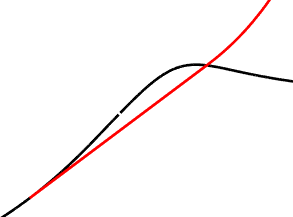
\includegraphics[width=4cm]{hs_generico(1)}};
%			%x
%			\draw[->,black] (0,0) -- (5,0) node [pos=1, above] {$s$};
%			%y
%			\draw[->,black] (0,0) -- (0,5) node [pos=1, right] {$h$};
%			\draw (3.68,3) -- (3.68,1.7) node [pos=1, right] {$h_2$};
%			\node at (4,3) {$h_1$};
%			\draw (3.68,1.7) -- (0.4,0.25) node [pos=1, above] {$h_0$};	
%	\end{tikzpicture}} \quad	
%	\subfloat{\scalebox{0.4}{\begin{tikzpicture}[>=latex]
%				%\draw [help lines] (0,0) grid (15,15);
%				% Generatore di Vapore con economizzatore
%				\draw (2,9) rectangle (4,11);
%				\draw [pattern=vertical lines] (2,8) rectangle (4,9);
%				% Surriscaldatore e collegamento turbina
%				\draw (3,11) -- (3,11.5) -- (3.5,12) -- (2.5,12.5) -- (3,13) -- (3,14) -- (9,14) -- (9,11);
%				% Turbina
%				\draw (9,11) -- (10,12) -- (10,9) -- (9,10) -- (9,11) -- cycle;
%				\draw [line width=3pt] (10, 10.5) -- (11, 10.5);
%				\node [draw, circle] at (11.35, 10.5) {$\sim$};
%				\draw (10,9) -- (10,8);
%				% Condensatore
%				\draw (10,7.5) circle (0.5cm);
%				\draw (11,8) -- (10,7.5) -- (11,7);
%				\draw (10,7) -- (10,5.5);
%				% Pompa di estrazione del condensato
%				\draw (10,5) circle (0.5cm);
%				\draw (10,4.5) -- (9.60,5.25) -- (10.40,5.25) -- cycle;
%				\draw [->] (10,4.5) -- (10,2);
%				% Serbatoio
%				\draw (11,2) -- (11,1) -- (8,1) -- (8,2);
%				\draw (11, 1.5) -- (8,1.5); 
%				\draw (8,1) -- (6,1);
%				% Pompa di Alimento
%				\draw (5.5,1) circle (0.5cm);
%				\draw (5,1) -- (5.75,1.4) -- (5.75,0.60) -- cycle;
%				\draw [->] (5,1) -- (3,1) -- (3,8);
%				% NOMI
%				\node at (3,10) {GV}; 
%				\node at (2,12) {SH};
%				\node at (9.5,10.5) {T};
%				\node at (11,7.5) {C};
%				\node at (11, 5) {Pe};
%				\node at (9.5, 0) {Serbatoio $H_2O$};
%				\node at (5.5, 0) {Pa};
%	\end{tikzpicture}}}
%\end{figure}


\begin{tikzpicture}
	\draw [help lines,step=.5] (0,0) grid (5,5);
	%x
	\draw[->] (0,0) -- (5,0) node [pos=1, above] {$\dot{m}$};
	%y
	\draw[->] (0,0) -- (0,5) node [pos=1, right] {$P_0$};
	\draw[thick, red] (0,4) -- (5,4) node [pos=0.5, above] {$GV$};
	\draw [blue](0,0) parabola (1,1);
	\draw [blue] (1,1) -- (4,5) node [pos=0.5, sloped, above] {Turbina};
	\draw[dashed] (0,1) -- (1,1);
	\draw[dashed] (1,0) -- (1,1);
	\draw[dashed] (3.25,4) -- (3.25,0) node [pos=1, below] {$\dot{m}^*$};
	\draw[teal] (1.5,4) -- (1.5,1.63) node [pos=0.5, left] {$\Delta P$};
	
\end{tikzpicture}
\end{document}